\section{COMPSs Tools}
\label{sec:Tools}

%%%%%%%%%%%%%%%%%%%%%%%%%%%%%%%%%%%%%%%%%%%%%%%%%%%%%%%
%%%%%%%%%%%%%%%%% APPLICATION GRAPH %%%%%%%%%%%%%%%%%%%
%%%%%%%%%%%%%%%%%%%%%%%%%%%%%%%%%%%%%%%%%%%%%%%%%%%%%%%
\subsection{Application graph}
At the end of the application execution a dependency graph can be generated representing the order of execution of each type of 
task and their dependencies. To allow the final graph generation the \textit{-g} flag has to be passed to the \textit{runcompss} command; the graph file is written in the \textit{$base\_log\_folder$}$/monitor/complete\_graph$.dot at the end of the execution.

Figure \ref{fig:complete_graph} shows a dependency graph example of a \textit{SparseLU} java application. The graph can be
visualized by running the following command:
\begin{lstlisting}[language=bash]
compss@bsc:~$ gengraph ~/.COMPSs/sparseLU.arrays.SparseLU_01/monitor/complete_graph.dot
\end{lstlisting}

\begin{figure}[h!]
  \centering
    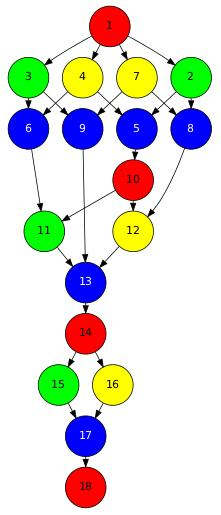
\includegraphics[width=0.3\textwidth]{./Sections/4_Tools/Figures/dependency_graph.jpeg}
    \caption{The dependency graph of the SparseLU application}
    \label{fig:complete_graph}
\end{figure}



%%%%%%%%%%%%%%%%%%%%%%%%%%%%%%%%%%%%%%%%%%%%%%%%%%%%%%%
%%%%%%%%%%%%%%%%%%%%%%%% MONITOR %%%%%%%%%%%%%%%%%%%%%%
%%%%%%%%%%%%%%%%%%%%%%%%%%%%%%%%%%%%%%%%%%%%%%%%%%%%%%%
\subsection{COMPSs Monitor}
\label{subsec:monitor}
The COMPSs Framework includes a Web graphical interface that can be used to monitor the execution of COMPSs applications. COMPSs Monitor is installed as a service and can be easily managed by running any of the following
commands:
\begin{lstlisting}[language=bash]
compss@bsc:~$ sudo service compss-monitor usage
Usage: /usr/sbin/service compss-monitor 
           {start | stop | reload | restart | try-restart | force-reload | status}
\end{lstlisting}

\subsubsection{Service configuration}
The COMPSs Monitor service can be configured by editing the \textit{/opt/COMPSs/Tools/}
\textit{monitor/apache-tomcat/conf/compss-monitor.conf}
file which contains one line per property:
\begin{itemize}
 \item \textbf{$IT\_MONITOR$} Default directory to retrieve monitored applications (defaults to the \textit{.COMPSs} folder inside the \textit{root} user).
 \item \textbf{$COMPSs\_MONITOR\_PORT$} Port where to run the compss-monitor web service (defaults to 8080).
 \item \textbf{$COMPSs\_MONITOR\_TIMEOUT$} Web page timeout between browser and server (defaults to 20s).
\end{itemize}

\subsubsection{Usage}
In order to use the COMPSs Monitor users need to start the service as shown in Figure \ref{fig:monitor_start}.
\begin{figure}[thb!]
  \centering
    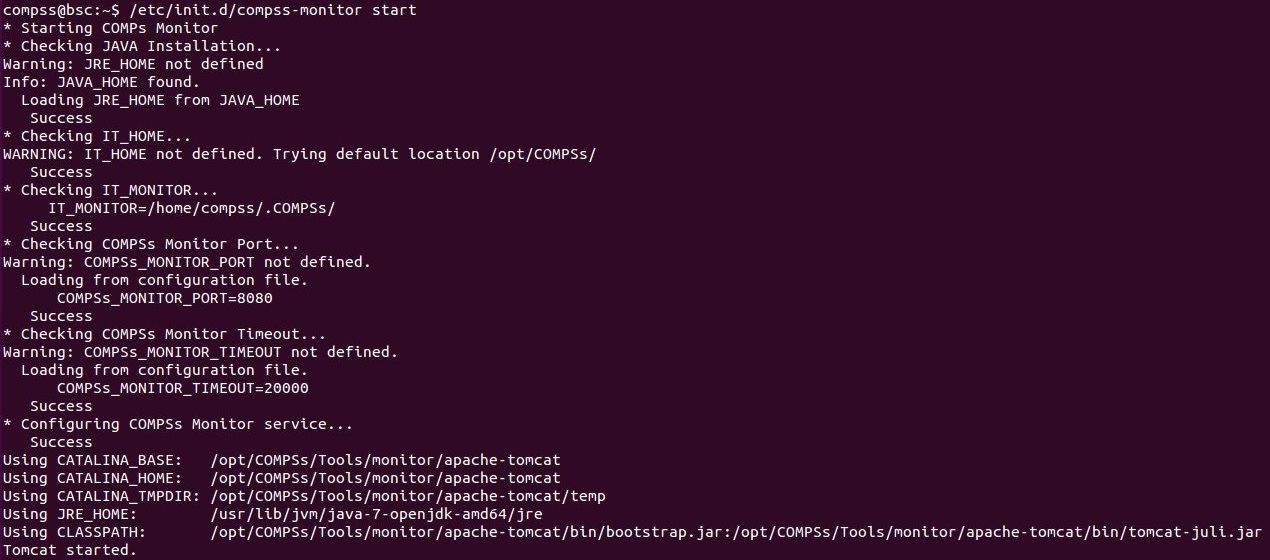
\includegraphics[width=\textwidth]{./Sections/4_Tools/Figures/monitor_start.jpeg}
    \caption{COMPSs Monitor start command}
    \label{fig:monitor_start}
\end{figure}

And use a web browser to open the specific URL:
\begin{lstlisting}[language=bash]
compss@bsc:~$ firefox http://localhost:8080/compss-monitor &
\end{lstlisting}

The COMPSs Monitor allows to monitor applications from different users and thus, users need to first login to access their applications. As shown in Figure \ref{fig:monitoring_interface}, the users can select any of their executed or running COMPSs applications and display it.
\begin{figure}[thb!]
  \centering
    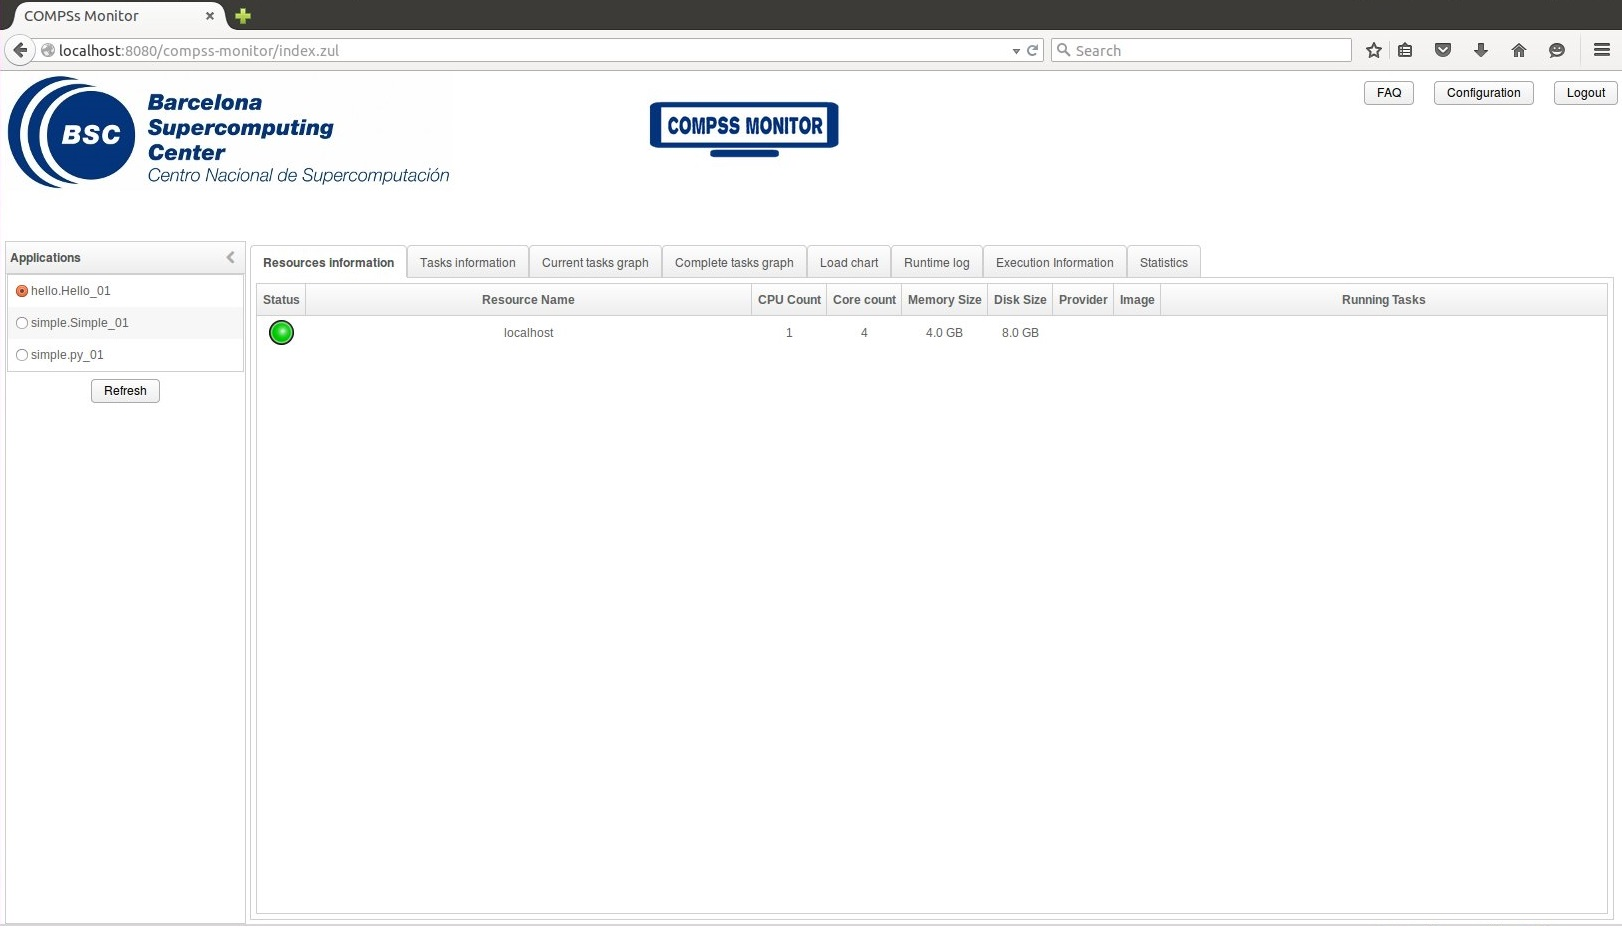
\includegraphics[width=0.95\textwidth]{./Sections/4_Tools/Figures/compss_monitor.jpeg}
    \caption{COMPSs monitoring interface}
    \label{fig:monitoring_interface}
\end{figure}

To enable \textbf{all} the COMPSs Monitor features, applications must run the runcompss command with the \textit{-m} flag. This flag 
allows the  COMPSs Runtime to store special information inside inside the \textit{log base folder} under the \textit{monitor} 
folder (see Figures \ref{fig:simple_exec_monitor} and \ref{fig:simple_logs_monitor}). Only advanced users should modify or delete any of these files. If the application that a user is trying to monitor 
has not been executed with this flag, some of the COMPSs Monitor features will be disabled. 
\begin{figure}[ht!]
  \centering
    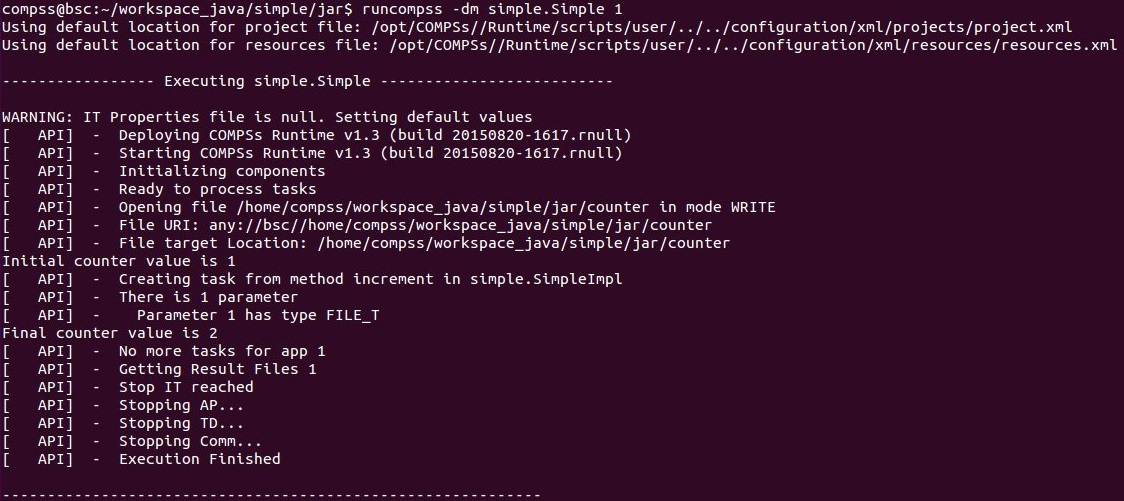
\includegraphics[width=0.95\textwidth]{./Sections/4_Tools/Figures/simple_monitor.jpeg}
    \caption{Execution of the Simple Java application with the monitoring flag enabled}
    \label{fig:simple_exec_monitor}
\end{figure}

\begin{figure}[ht!]
  \centering
    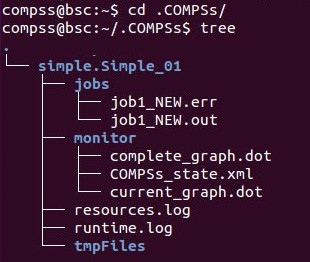
\includegraphics[width=0.4\textwidth]{./Sections/4_Tools/Figures/logs_with_monitor.jpeg}
    \caption{Logs generated by the Simple java application with the monitoring flag enabled}
    \label{fig:simple_logs_monitor}
\end{figure}

\newpage
\subsubsection{Graphical Interface features}
In this section we provide a summary of the COMPSs Monitor supported features available through the graphical interface:
\begin{itemize}
 \item \textbf{Resources information} \newline
	Provides information about the resources used by the application
 \item \textbf{Tasks information} \newline
	Provides information about the tasks definition used by the application
 \item \textbf{Current tasks graph} \newline
	Shows the tasks dependency graph currently stored into the COMPSs Runtime
 \item \textbf{Complete tasks graph} \newline
	Shows the complete tasks dependecy graph of the application
 \item \textbf{Load chart} \newline
	Shows different dynamic charts representing the evolution over time of the resources load and the tasks load
 \item \textbf{Runtime log} \newline
	Shows the runtime log
 \item \textbf{Execution Information} \newline
	Shows specific job information allowing users to easily select failed or uncompleted jobs
 \item \textbf{Statistics} \newline
	Shows application statistics such as the accumulated cloud cost. 
\end{itemize}

\colorComment{\textbf{Attention}: To enable all the COMPSs Monitor features applications must run with the \textit{$-m$} flag.}

The webpage also allows users to configure some performance parameters of the monitoring service by accessing the 
\textit{Configuration} button at the top-right corner of the web page. 

For specific COMPSs Monitor feature configuration please check our \textit{FAQ} section at the top-right corner of the web page. 


%%%%%%%%%%%%%%%%%%%%%%%%%%%%%%%%%%%%%%%%%%%%%%%%%%%%%%%
%%%%%%%%%%%%%%%% APPLICATION TRACING %%%%%%%%%%%%%%%%%%
%%%%%%%%%%%%%%%%%%%%%%%%%%%%%%%%%%%%%%%%%%%%%%%%%%%%%%%
\subsection{Application tracing}
\label{sec:Tracing}
COMPSs Runtime can generate a post-execution trace of the execution of the application. This trace is useful for
performance analysis and diagnosis.

A trace file may contain different events to determine the COMPSs master state, the task execution state or the file-transfers.
The current release does not support file-transfers informations.

During the execution of the application, an XML file is created in the worker nodes to keep track of 
these events. At the end of the execution, all the XML files are merged to get a final trace file.

In this manual we only provide information about how to obtain a trace and about the available Paraver (the tool used to analyze the traces) configurations. For further
information about the application instrumentation or the trace visualization please check the \textit{COMPSs Tracing Manual} 
available at \url{http://compss.bsc.es} .

\subsubsection{Trace Command}
In order to obtain a post-execution trace file the option \textbf{-t}  must be added to the runcompss command. Next we provide an
example of the command execution with the tracing option enabled for the Hmmer java application.

\begin{lstlisting}[language=bash]
compss@bsc:~$ runcompss -t --classpath=/home/compss/workspace_java/hmmerobj/jar/hmmerobj.jar 
                        hmmerobj.HMMPfam 
                        /sharedDisk/Hmmer/smart.HMMs.bin /sharedDisk/Hmmer/256seq 
                        /home/compss/out.txt 2 8 -A 222

----------------- Executing hmmerobj.HMMPfam --------------------------

WARNING: IT Properties file is null. Setting default values
Welcome to Extrae 3.1.1rc (revision 3360 based on extrae/trunk)
Extrae: Warning! EXTRAE_HOME has not been defined!.
Extrae: Generating intermediate files for Paraver traces.
Extrae: Intermediate files will be stored in /home/compss/workspace_java/hmmerobj/jar
Extrae: Tracing buffer can hold 500000 events
Extrae: Tracing mode is set to: Detail.
Extrae: Successfully initiated with 1 tasks

Extrae: Warning! API tries to initialize more than once
Extrae:          Previous initialization was done by API

[   API]  -  Starting COMPSs Runtime v1.3 (build 20151016-1931.rnull)

...
...
...

[   API]  -  No more tasks for app 1
[   API]  -  Getting Result Files 1
[   API]  -  Execution Finished

Extrae: Intermediate raw trace file created : /home/compss/workspace_java/hmmerobj/jar/set-0/TRACE@bsc.0000031637000000000000.mpit
Extrae: Intermediate raw sym file created : /home/compss/workspace_java/hmmerobj/jar/set-0/TRACE@bsc.0000031637000000000000.sym
Extrae: Deallocating memory.
Extrae: Application has ended. Tracing has been terminated.

merger: Output trace format is: Paraver
merger: Extrae 3.1.1rc (revision 3360 based on extrae/trunk)

mpi2prv: Checking for target directory existance... exists, ok!
mpi2prv: Selected output trace format is Paraver
mpi2prv: Stored trace format is Paraver
mpi2prv: Parsing intermediate files
mpi2prv: Removing temporal files... done
mpi2prv: Congratulations! ./trace/hmmerobj.HMMPfam_compss_trace_1440151114.prv has been generated.

------------------------------------------------------------
\end{lstlisting}

At the end of the execution the trace will be stored inside the \textit{trace} folder under the application log directory.
\begin{lstlisting}[language=bash]
compss@bsc:~$ cd .COMPSs/hmmerobj.HMMPfam/trace/
compss@bsc:~$ ls -1
hmmerobj.HMMPfam_compss_trace_1444922077.pcf
hmmerobj.HMMPfam_compss_trace_1444922077.prv
hmmerobj.HMMPfam_compss_trace_1444922077.row
\end{lstlisting}


\subsubsection{Trace Configurations}
The traces generated by an application execution are ready to be visualized with \textit{Paraver}. \textit{Paraver} is a powerful 
tool developed by \textit{BSC} that allows users to show many views of the trace data by means of different configuration files.
Users can manually load, edit or create configuration files to obtain different trace data views.

In Table \ref{tab:paraver_configs} we provide information about the different pre-build configurations that we distribute
with COMPSs and that can be found under the \textit{/opt/COMPSs/Dependencies/paraver/cfgs/} folder.

\bgroup
  \def\arraystretch{1.5}
  \begin{table}[h]
    \begin{center}
      \begin{tabular}{| p{0.45\textwidth} | p{0.45\textwidth} |}
	\hline
	$2dp\_runtime\_state.cfg$		& 2D plot of runtime state \\ \hline
	$2dp\_tasks.cfg$			& 2D plot of tasks duration \\ \hline
	$3dh\_duration\_runtime.cfg$		& 3D Histogram of runtime execution \\ \hline
	$3dh\_duration\_tasks.cfg$		& 3D Histogram of tasks duration \\ \hline
	$compss\_runtime.cfg$ 			& Shows COMPSs Runtime events (at master and workers) \\ \hline
	$compss\_tasks\_and\_runtime.cfg$ 	& Shows COMPSs Runtime events (at master and workers) and tasks execution \\ \hline
	$compss\_tasks.cfg$ 			& Shows tasks execution \\ \hline
	$compss\_tasks\_numbers.cfg$ 		& Shows tasks execution by task id \\ \hline
	$compss\_transfers.cfg$ 		& Shows transfer time spent by each worker \\ \hline
      \end{tabular}
      \caption{Available paraver configurations for COMPSs Applications}
      \label{tab:paraver_configs}
    \end{center}
  \end{table}
\egroup

For further information about \textit{Paraver} please visit the following site:
\begin{center}
\url{http://www.bsc.es/computer-sciences/performance-tools/paraver}
\end{center}


\subsubsection{Trace examples}
COMPSs traces can be very complex as the number of workers or tasks grows. Just to illustrate this, the following 
pictures show traces with a greater number of workers and tasks.

\begin{figure}[ht!]
  \centering
    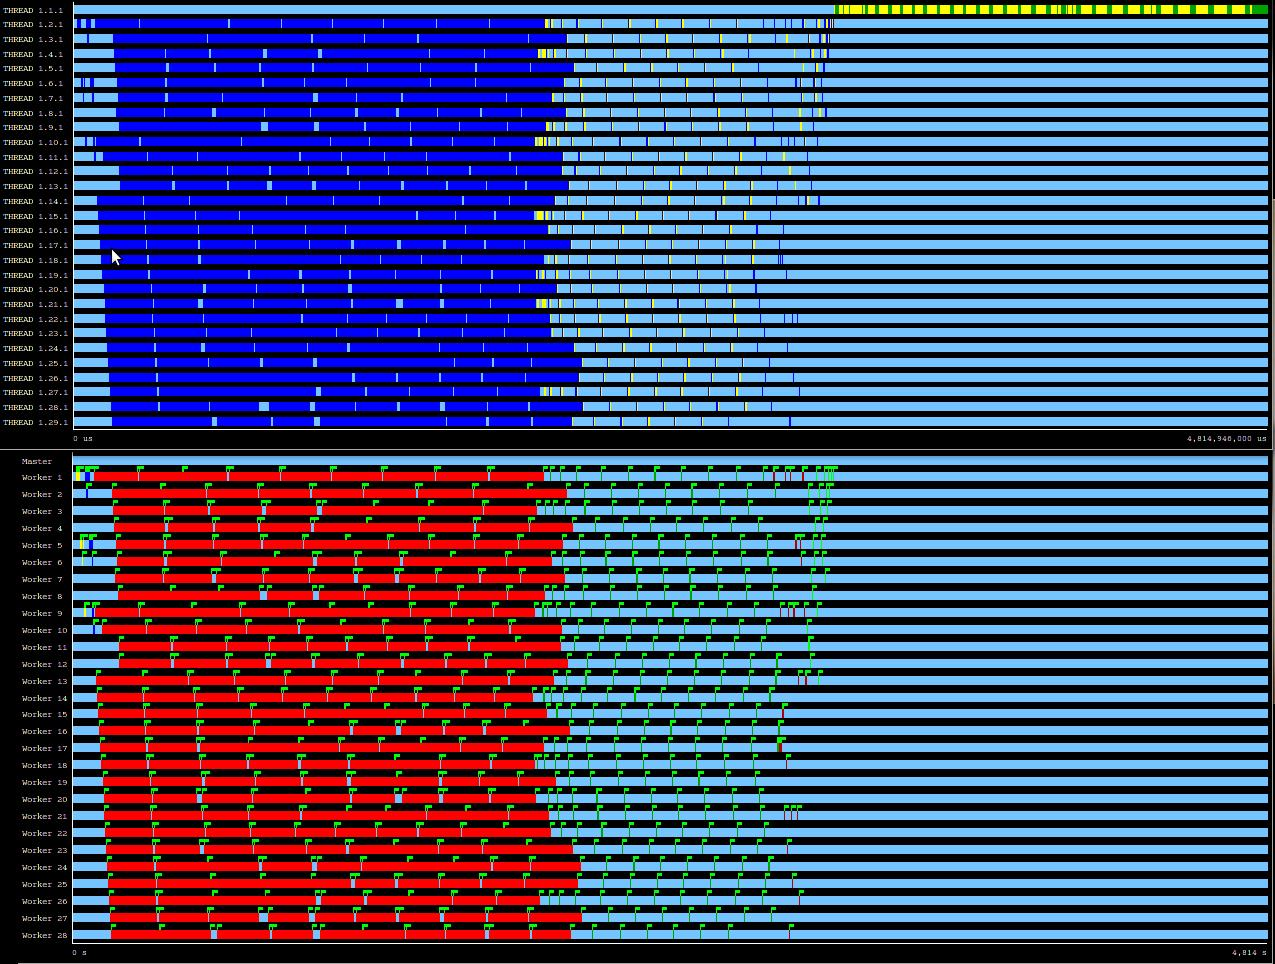
\includegraphics[width=0.91\textwidth]{./Sections/4_Tools/Figures/trace_example1.jpeg}
    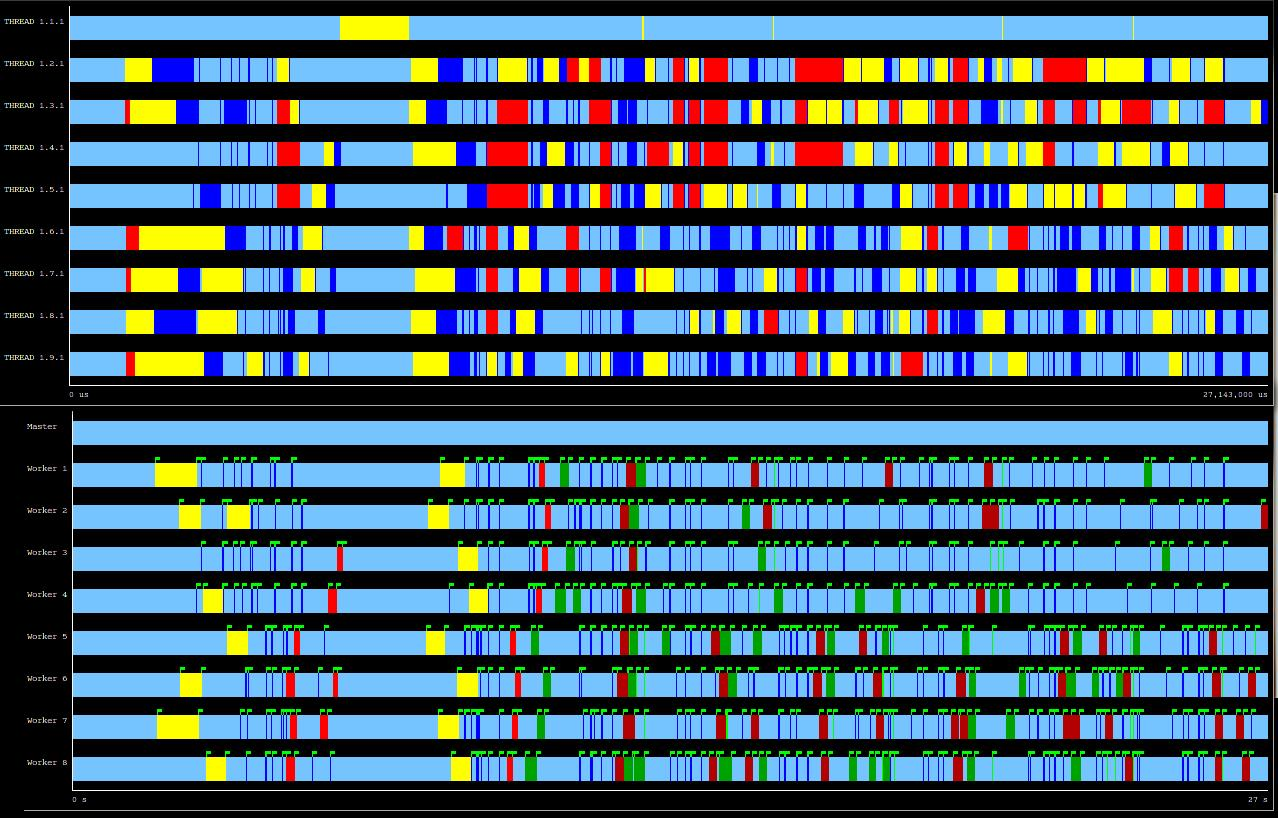
\includegraphics[width=0.91\textwidth]{./Sections/4_Tools/Figures/trace_example2.jpeg}
    \caption{Examples of complex traces}
\end{figure}

\newpage
%%%%%%%%%%%%%%%%%%%%%%%%%%%%%%%%%%%%%%%%%%%%%%%%%%%%%%%
%%%%%%%%%%%%%%%%%%%%%%%%% IDE %%%%%%%%%%%%%%%%%%%%%%%%%
%%%%%%%%%%%%%%%%%%%%%%%%%%%%%%%%%%%%%%%%%%%%%%%%%%%%%%%
\subsection{COMPSs IDE}
\label{subsec:IDE}
COMPSs IDE is an Integrated Development Environment to develop, compile, deploy and execute COMPSs applications. It is available
through the \textit{Eclipse Market} as a plugin and provides an even easier way to work with COMPSs.

For further information please check the \textit{COMPSs IDE User Guide} available at: \url{http://compss.bsc.es} .
